\documentclass[12pt, aspectratio=169]{beamer}

\input{../header}
\usepackage{booktabs}
\DeclareMathOperator{\E}{E}
\DeclareMathOperator{\V}{V}

\title{Test of Hypothesis}
\author{Md. Aminul Islam Shazid}
\date{}


\begin{document}
    {
		\setbeamertemplate{footline}{}
		\addtocounter{framenumber}{-2}

		\begin{frame}
			\titlepage
		\end{frame}

		\begin{frame}{Outline}
            \vfill
			\tableofcontents[subsectionstyle=hide]
            \vfill
		\end{frame}
	}

    \section{Introduction}


    \begin{frame}{Test of Hypothesis - Overview}
        \begin{itemize}
            \item A statistical hypothesis is a claim about a population parameter (population mean, population proportion, population variance etc.)
            \item We test this claim using sample data
            \item The goal is to make a decision under uncertainty
            \item Decisions are made using probability and sampling distributions
        \end{itemize}
    \end{frame}


    \begin{frame}{Statistical Hypotheses}
        \begin{itemize}
            \item \textbf{Null hypothesis ($H_0$):} baseline assumption
            \item \textbf{Alternative hypothesis ($H_A$):} competing claim
            \item They are mutually exclusive and exhaustive
            \item Example:
            \[
            H_0: \mu = 100 \quad \text{vs} \quad H_A: \mu \neq 100
            \]
            \item We use sample to assess whether the data provides any evidence \emph{against} the null hypothesis
            \item Based on the available data, we either reject the null hypothesis in favor of the alternative or ``fail to reject the null hypothesis"
            \item Therefore, we do not ``accept'' the null hypothesis
        \end{itemize}
    \end{frame}


    \begin{frame}{Types of Tests (Alternative Hypotheses)}
        \begin{itemize}
            \item Two-tailed:
            \[
            H_A: \mu \neq \mu_0
            \]
            \item Left-tailed:
            \[
            H_A: \mu < \mu_0
            \]
            \item Right-tailed:
            \[
            H_A: \mu > \mu_0
            \]
        \end{itemize}
    \end{frame}


    \section{Types of Errors}


    \begin{frame}{Type I Error}
        \begin{itemize}
            \item Rejecting $H_0$ when it is true
            \item Probability of type I error (also known as \emph{level of significance}):
            \[
            \alpha = P(\text{Reject } H_0 \mid H_0 \text{ true})
            \]
            \item Also called false positive
        \end{itemize}
    \end{frame}


    \begin{frame}{Type II Error}
        \begin{itemize}
            \item Failing to reject $H_0$ when it is false
            \item Probability of type II error:
            \[
            \beta = P(\text{Fail to reject } H_0 \mid H_0 \text{ false})
            \]
            \item Also called false negative
        \end{itemize}
    \end{frame}


    \begin{frame}{Errors Summary Table}
        \begin{center}
            \begin{tabular}{c|cc}
                \hline
                & $H_0$ True & $H_0$ False \\
                \hline
                Reject $H_0$ & Type I & Correct \\
                Fail to reject $H_0$ & Correct & Type II \\
                \hline
            \end{tabular}
        \end{center}
    \end{frame}


    % \section{Significance Level and Power}


    \begin{frame}{Level of Significance}
        \begin{itemize}
            \item $\alpha = P(\text{Type I error}) = P(\text{Reject } H_0 \mid H_0 \text{ true})$
            \item Common choices: $0.10,\ 0.05,\ 0.01$
            \item It is essentially our ``tolerance'' for type I error
            \item Smaller choice of $\alpha$ means stricter evidence required
        \end{itemize}
    \end{frame}


    \begin{frame}{Choosing $\alpha$ in Practice}
        \begin{itemize}
            \item There is no universally ``correct'' $\alpha$ --- the choice should reflect how costly a Type I error is in the given context
            \item Use a \textbf{stricter (smaller) $\alpha$} (e.g. $0.01$) when a false positive is dangerous or expensive
            \begin{itemize}
                \item Example: approving a new drug as safe when it is not; certifying a structural design as safe when it is not
            \end{itemize}
            \item Use a \textbf{looser (larger) $\alpha$} (e.g. $0.10$) when missing a real effect is costlier than a false alarm
            \begin{itemize}
                \item Example: early-stage screening for a promising material or drug candidate
            \end{itemize}
            \item $\alpha = 0.05$ is the conventional default when there is no strong reason to move away from it
        \end{itemize}
    \end{frame}


    \begin{frame}{Power of a Test}
        \begin{itemize}
            \item \textbf{Power} is the probability of correctly rejecting $H_0$
                when it is actually false
            \[
                \text{Power} = 1 - \beta = P(\text{Reject } H_0 \mid H_0 \text{ false})
            \]
            \item A test with low power may fail to reject a false \(H_0\), a \emph{false negative} error
            \item Power depends on:
            \begin{itemize}
                \item \textbf{Sample size} $n$: larger $n$ $\Rightarrow$ higher power
                \item \textbf{Effect size} $|\mu - \mu_0|$: larger effect $\Rightarrow$ easier to detect
                \item \textbf{Variability} $\sigma$: smaller $\sigma$ $\Rightarrow$ higher power
                \item \textbf{Significance level} $\alpha$: larger $\alpha$ $\Rightarrow$ higher power (but at the cost of higher Type I error probability)
            \end{itemize}
            \item Conventionally, power $\geqslant 0.80$ is considered adequate
        \end{itemize}
    \end{frame}


    \begin{frame}{Choosing Sample Size via Power}
        \begin{itemize}
            \item Sample size should be decided \textbf{before} data collection, not after
            \item Given a target power (typical convention is to set power at $0.80$), the minimum required $n$ can be calculated
            % \item Rule of thumb: smaller effect size or larger $\sigma$ $\Rightarrow$ larger $n$ needed to keep power adequate
            \item Larger $n$ costs more time and resources, but too small an $n$ can lead too too low power (a high $\beta$)
            \item In practice, this calculation is done using statistical software (power analysis), not by hand
        \end{itemize}
    \end{frame}


    \begin{frame}{Test Outcomes and Their Probabilities}
        \begin{center}
            \begin{tabular}{c|cc}
                \hline
                & $H_0$ True & $H_0$ False \\
                \hline
                Reject $H_0$ & Type I ($\alpha$) & Correct ($1-\beta$) \\
                Fail to reject $H_0$ & Correct ($1-\alpha$) & Type II ($\beta$) \\
                \hline
            \end{tabular}
        \end{center}

        \begin{itemize}
            \item \(\alpha = \) level of significance
            \item \(1 - \beta = \) power of a test
        \end{itemize}
    \end{frame}


    \section{Test about a Single Mean}


    \begin{frame}{Test about a Single Mean --- Test Statistic}
        \begin{itemize}
            \item Used to test a claim about a population mean $\mu$ based on a sample mean $\bar{x}$
            \item \textbf{Test statistic:}
            \[
                t_{\text{cal}} = \frac{\bar{x} - \mu_0}{s/\sqrt{n}} \sim t_{n-1} \quad \text{under } H_0
            \]
            \item The $t$-test is used regardless of sample size --- it converges to the $Z$-test for large $n$, but remains valid and more robust for small $n$
        \end{itemize}
    \end{frame}


    \begin{frame}{Test about a Single Mean --- Example}
        \textbf{Problem:} It is claimed that the mean weight of teens in a city
        is 35\,kg. A sample of $n = 10$ teens yields $\bar{x} = 40.1$\,kg,
        $s = 4.2$\,kg. At $\alpha = 0.05$, does the mean weight differ from 35\,kg?

        \vspace{0.8em}

        Let $\mu = $ mean weight of the teens.

        \[
            H_0: \mu = 35 \quad \text{vs} \quad H_A: \mu \neq 35
        \]

        \vspace{0.5em}

        \textbf{Assumptions:} Population is normally distributed; $\sigma$ unknown.
    \end{frame}


    \begin{frame}{Test about a Single Mean --- Solution}
        \begin{columns}
            \begin{column}{0.55\textwidth}
                \textbf{Test statistic:}
                \[
                    t_{\text{cal}} = \frac{\bar{x} - \mu_0}{s/\sqrt{n}}
                    = \frac{40.1 - 35}{4.2/\sqrt{10}} = 3.84
                \]
                \textbf{Critical value:} $t_{0.025,\,9} = 2.262$

                \vspace{0.25em}

                \textbf{Decision:} Since $t_{\text{cal}} = 3.84 > 2.262$,
                we \textbf{reject} $H_0$ at 5\% level of significance.

                \vspace{0.25em}

                % \textbf{P-value:}
                % \[
                %     p = 2\,P(t_9 \geqslant 3.84) \approx 0.004
                % \]
                % Since $p = 0.004 < \alpha = 0.05$, we reject $H_0$.
                There is strong evidence that the mean weight differs from 35\,kg.
            \end{column}
            \begin{column}{0.45\textwidth}
                \begin{center}
                    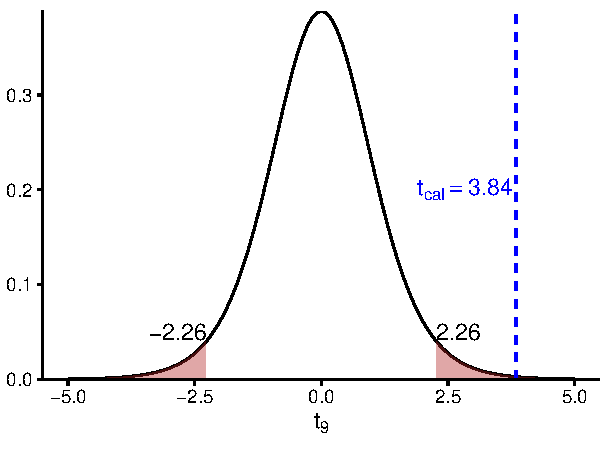
\includegraphics[width=\textwidth]{plots/single-mean-t-test.pdf}
                \end{center}
            \end{column}
        \end{columns}
    \end{frame}


    \section{Test about Two Means (Independent Samples)}


    \begin{frame}{Two Means (Independent, Equal Variances) --- Test Statistic}
        \begin{itemize}
            \item Used to compare the means of two \textbf{independent} populations, assuming equal population variances ($\sigma_1^2 = \sigma_2^2$)
            \item \textbf{Pooled variance:}
            \[
                S^2 = \frac{(n_1-1)S_1^2 + (n_2-1)S_2^2}{n_1+n_2-2}
            \]
            \item \textbf{Test statistic:}
            \[
                t_{\text{cal}} = \frac{\bar{x}_1 - \bar{x}_2}{S\sqrt{\tfrac{1}{n_1}+\tfrac{1}{n_2}}}
                \sim t_{n_1+n_2-2} \quad \text{under } H_0
            \]
        \end{itemize}
    \end{frame}


    \begin{frame}{Two Means (Independent, Equal Variances) --- Example}
        \textbf{Problem:} A sample of 9 bulbs from Company~A had a mean lifetime of
        1309\,hrs ($s_1 = 419$); a sample of 16 bulbs from Company~B had a mean of
        1205\,hrs ($s_2 = 390$).
        Do the two companies' bulbs differ significantly in mean lifetime?
        Use $\alpha = 0.05$. Assume \textbf{equal} population variances.

        \vspace{0.8em}

        Let $\mu_1, \mu_2 = $ mean lifetimes of bulbs from Company A and B respectively.

        \[
            H_0: \mu_1 = \mu_2 \quad \text{vs} \quad H_A: \mu_1 \neq \mu_2
        \]
    \end{frame}


    \begin{frame}{Two Means (Independent, Equal Variances) --- Solution}
        \begin{columns}
            \begin{column}{0.55\textwidth}
                \textbf{Pooled variance:}
                \[
                    S^2 = \frac{8\times 419^2 + 15\times 390^2}{23} = 160260.3
                \]

                \textbf{Test statistic:}
                \[
                    t_{\text{cal}} = \frac{1309 - 1205}{S\sqrt{\tfrac{1}{9}+\tfrac{1}{16}}}
                    = 0.623
                \]

                \textbf{Critical value:} $t_{0.025,\,23} = 2.069$

                \vspace{0.25em}

                \textbf{Decision:} Since $|t_{\text{cal}}| = 0.623 < 2.069$,
                we \textbf{fail to reject} $H_0$ at 5\% level of significance.
                There is no significant difference between the mean lifetimes.
            \end{column}
            \begin{column}{0.45\textwidth}
                \begin{center}
                    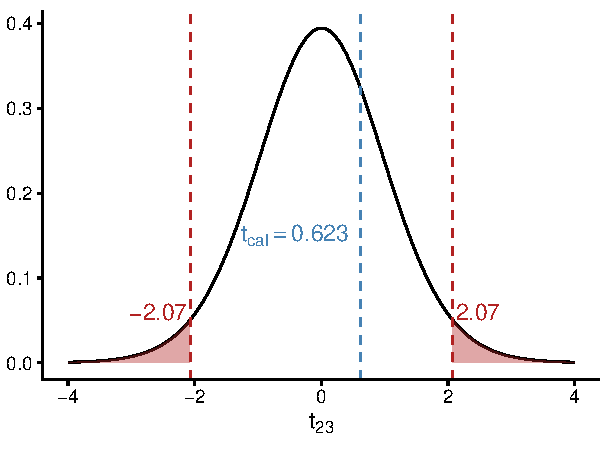
\includegraphics[width=\textwidth]{plots/two-mean-indep-equal.pdf}
                \end{center}
            \end{column}
        \end{columns}
    \end{frame}


    \section{Test about Two Means (Dependent Samples)}


    \begin{frame}{Test about Two Means --- Dependent (Paired) Samples}
        \begin{itemize}
            \item Used when the two samples are \textbf{not independent}
            \item Common when the same subjects are measured \textbf{before and after}
                a treatment, or under two conditions
            \item Define the \textbf{difference}: $d_i = x_i - y_i$
            \item This reduces the two-sample problem to a \textbf{one-sample}
                $t$-test on the differences
        \end{itemize}

        \vspace{0.5em}

        \textbf{Test statistic:}
        \[
            t_{\text{cal}} = \frac{\bar{d}}{s_d/\sqrt{n}} \sim t_{n-1}
            \quad \text{under } H_0
        \]

        where $\bar{d} = \frac{\sum d_i}{n}$ and
        $s_d^2 = \frac{1}{n-1}\left(\sum d_i^2 - \frac{(\sum d_i)^2}{n}\right)$
    \end{frame}


    \begin{frame}{Two Means (Dependent) --- Example}
        \textbf{Problem:} Nine adults agreed to test a new diet program.
        Their weights (in lb) were recorded before and after the program.
        Test whether the program is effective in reducing weight at $\alpha = 0.05$.

        \vspace{0.5em}

        \begin{center}
            \small
            \begin{tabular}{lccccccccc}
                \toprule
                & \multicolumn{9}{c}{\textbf{Adult}} \\
                \cmidrule{2-10}
                & 1 & 2 & 3 & 4 & 5 & 6 & 7 & 8 & 9 \\
                \midrule
                Before ($x_i$) & 132 & 138 & 126 & 114 & 122 & 132 & 142 & 119 & 137 \\
                After ($y_i$) & 130 & 132 & 130 & 111 & 122 & 133 & 139 & 119 & 130 \\
                \bottomrule
            \end{tabular}
        \end{center}

        \[
            H_0: \mu_d = 0 \quad \text{vs} \quad H_A: \mu_d > 0
        \]
    \end{frame}


    \begin{frame}{Two Means (Dependent) --- Solution}
        \begin{columns}
            \begin{column}{0.55\textwidth}
                \textbf{Summary statistics:}
                \(
                    \bar{d} = \frac{4}{9} = 0.44, \qquad s_d^2 = 21.53
                \)

                \vspace{0.25em}

                \textbf{Test statistic:}
                \[
                    t_{\text{cal}} = \frac{0.44}{4.64/\sqrt{9}} = 0.28
                \]

                \textbf{Critical value:} $t_{0.05,\,8} = 1.86$

                \vspace{0.25em}

                \textbf{Decision:} Since $t_{\text{cal}} = 0.28 < 1.86$,
                we \textbf{fail to reject} $H_0$ at 5\% level of significance.

                \vspace{0.25em}

                \textbf{Conclusion:} There is insufficient evidence to conclude
                that the new diet program reduces weight.
            \end{column}
            \begin{column}{0.45\textwidth}
                \begin{center}
                    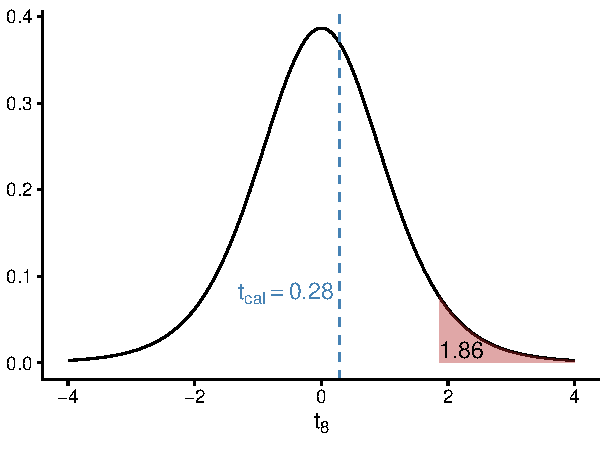
\includegraphics[width=\textwidth]{plots/paired-t-test.pdf}
                \end{center}
            \end{column}
        \end{columns}
    \end{frame}


    % \section{Chi-Square Test of Association}


    % \begin{frame}{Chi-Square Test of Association}
    %     \begin{itemize}
    %         \item Used to test whether two \textbf{categorical variables} are associated, based on data in an $r \times c$ \textbf{contingency table} of observed frequencies $O_{ij}$
    %         \item Hypotheses:
    %         \[
    %             H_0: \text{the two variables are independent} \quad \text{vs} \quad H_A: \text{the two variables are associated}
    %         \]
    %         \item Expected frequency under $H_0$:
    %         \[
    %             E_{ij} = \frac{(\text{row } i \text{ total}) \times (\text{column } j \text{ total})}{n}
    %         \]
    %         \item Test statistic:
    %         \[
    %             \chi^2_{\text{cal}} = \sum_{i}\sum_{j} \frac{(O_{ij}-E_{ij})^2}{E_{ij}} \sim \chi^2_{(r-1)(c-1)} \quad \text{under } H_0
    %         \]
    %         \item A large $\chi^2_{\text{cal}}$ means the observed frequencies deviate substantially from what independence would predict
    %     \end{itemize}
    % \end{frame}


    % \begin{frame}{Chi-Square Test of Association --- Example}
    %     \textbf{Problem:} A study of 200 patients records whether they are
    %     smokers and whether they have a respiratory disorder. Is smoking
    %     status associated with the disorder? Use $\alpha = 0.05$.

    %     \vspace{0.5em}

    %     \begin{center}
    %         \begin{tabular}{lccc}
    %             \toprule
    %             & \textbf{Disorder: Yes} & \textbf{Disorder: No} & \textbf{Total} \\
    %             \midrule
    %             Smoker & 45 & 55 & 100 \\
    %             Non-smoker & 20 & 80 & 100 \\
    %             \midrule
    %             Total & 65 & 135 & 200 \\
    %             \bottomrule
    %         \end{tabular}
    %     \end{center}

    %     \vspace{0.5em}

    %     \[
    %         H_0: \text{smoking status and disorder are independent} \quad \text{vs} \quad H_A: \text{they are associated}
    %     \]
    % \end{frame}


    % \begin{frame}{Chi-Square Test of Association --- Solution}
    %     \begin{columns}
    %         \begin{column}{0.55\textwidth}
    %             \textbf{Expected frequencies:}
    %             \[
    %                 E_{11} = E_{21} = \frac{100 \times 65}{200} = 32.5, \quad
    %                 E_{12} = E_{22} = \frac{100 \times 135}{200} = 67.5
    %             \]

    %             \textbf{Test statistic:}
    %             \[
    %                 \chi^2_{\text{cal}} = \frac{(45-32.5)^2}{32.5} + \frac{(55-67.5)^2}{67.5}
    %                 + \frac{(20-32.5)^2}{32.5} + \frac{(80-67.5)^2}{67.5} = 14.25
    %             \]

    %             \textbf{Critical value:} $\chi^2_{0.05,\,1} = 3.841$

    %             \vspace{0.25em}

    %             \textbf{Decision:} Since $\chi^2_{\text{cal}} = 14.25 > 3.841$,
    %             we \textbf{reject} $H_0$ at 5\% level of significance.
    %             Smoking status and the respiratory disorder are associated.
    %         \end{column}
    %         \begin{column}{0.45\textwidth}
    %             \phantom{.}
    %             \vspace{3em}
    %             \begin{center}
    %                 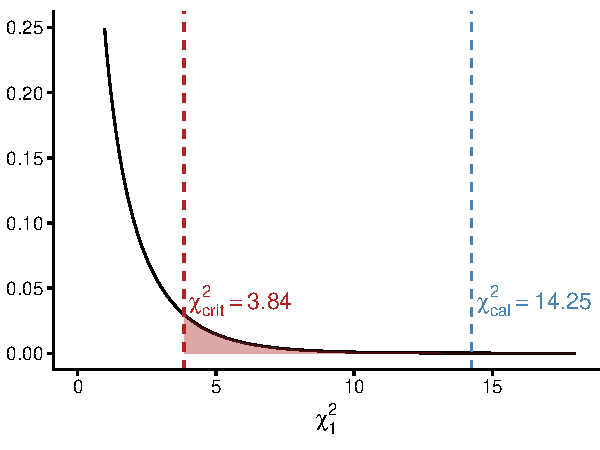
\includegraphics[width=\textwidth]{plots/chi-square-association.pdf}
    %             \end{center}
    %         \end{column}
    %     \end{columns}
    % \end{frame}


    
    \section{P-value}

    \begin{frame}{P-value: Meaning and Decision Rule}
        \begin{itemize}
            \item The \textbf{p-value} is the probability of observing a test statistic
                as extreme as, or more extreme than, the one calculated from the sample ---
                \emph{assuming $H_0$ is true}
            \item It is \textbf{not} the probability that $H_0$ is true
            \item A \textbf{small} p-value means the observed data would be very
                unlikely if $H_0$ were true --- evidence against $H_0$
            \item A \textbf{large} p-value means the data are consistent with $H_0$, but this does \emph{not} prove $H_0$ is true
            \item Decision rule:
            \begin{itemize}
                \item $p \leqslant \alpha$: reject $H_0$
                \item $p > \alpha$: fail to reject $H_0$
            \end{itemize}
            \item P-value is reported statistical software, and usually not calculated by hand
        \end{itemize}
    \end{frame}


    \section*{Thank you.}

\end{document}
